 \documentclass[a4paper]{article}

%% Language and font encodings
\usepackage[spanish]{babel}
\usepackage{fontspec}

%% Sets page size and margins
\usepackage[a4paper,top=3cm,bottom=2cm,left=3cm,right=3cm,marginparwidth=1.75cm]{geometry}

%% Useful packages
\usepackage{amsmath,amsthm,amssymb,amsfonts}
\usepackage{graphicx}
\usepackage[colorinlistoftodos]{todonotes}
\usepackage[colorlinks=true, allcolors=blue]{hyperref}
\usepackage{braket}
\usepackage{enumitem}


\newcommand{\R}{\mathbb{R}}
\newcommand{\N}{\mathbb{N}}
\newcommand{\Z}{\mathbb{Z}}
\providecommand{\C}{\mathbb{C}}

\theoremstyle{definition}
\newtheorem{defin}{Definición}

\theoremstyle{plain}
\newtheorem{theorem}[defin]{Teorema}
\newtheorem{corollary}[defin]{Corolario}



\title{Proyecto Mecánica cuántica\\ Física Computacional I}

\author{Daniela Andrea Torres Gómez\\ C.C 1.036.665.120

}

\date{}

\begin{document}
\maketitle

%\begin{abstract}
%Your abstract.
%\end{abstract}


\section*{Pozo Finito de Potencial}

\begin{figure}
\begin {center}
\includegraphics[width=0.50\textwidth]{finitewall.png}
\caption{Esquema del problema del pozo finito de potencial}

\label{fig:finitewall}
\end {center}
\end{figure}

Se la ecuación de Schrödinger unidimensional independiente del tiempo:

\begin{equation}
    \frac{-\hslash^2}{2m} \frac{d^2}{dz} \Psi(z) + V(z) \Psi(z) = E \Psi(z)
    \label{ec_1}
\end{equation}

Para una partícula en un pozo finito de potencial $V(z)$, tal que:
\\
$$V(z) = 
\begin{cases}
0, |z| \leq a/2 \\
V_o, |z| > a/2
\end{cases}
$$


\rule{145 mm}{0.1 mm}

\section{Solución Teórica}
- Regiones I y II de la figura \ref{fig:finitewall}:
La ecuación de Schrödinger queda como: 

\begin{align*}
    \Psi''(z) &= \frac{(V_o-E)}{2m \hslash^2} \Psi(z) \\
    &= k_o^2  \Psi(z)
\end{align*}

Para que es sistema sea ligado, la energía de la partícula debe cumplir $E<V_o$ y por lo tanto $(V_o - E)>0$, de otra forma sería el caso de una partícula libre. Además se definió el número de onda es $k_o = \sqrt{\frac{2m (V_o-E)}{\hslash^2}} $

Y las soluciones en cada región son:
$$
\begin{cases}
\Psi_I(x, t) = A e^{ k_o z} + Be^{- k_o z} \\
\Psi_{III}(x, t) = A' e^{k_o z} + B' e^{-k_o z}
\end{cases}
$$


- Región II:
La ecuación de Schrödinger queda como: 

\begin{align*}
    \Psi''(z) &= -\frac{E}{2m \hslash^2} \Psi(z)\\
    &= - k_1^2  \Psi(z)
\end{align*}

donde el número de onda es $k_1 = \sqrt{\frac{2m E}{\hslash^2}} $

Y la solución es:

\begin{align*}
    \Psi_{II}(x, t) = C \cos(k_1 z) + D \sin(k_1 z)
\end{align*}

Las condicione de frontera consideran que $\Psi$ es continua en toda la región, y cómo la barrera de potencial es finita, entonces su derivada espacial $d\Psi/dz$ también es continua. Es decir:

$$
\begin{cases}
\Psi_I(-a/2) = \Psi_{II}(-a/2) \\
\Psi_{II}(a/2) = \Psi_{III}(a/2) \\
\Psi'_I(-a/2) = \Psi'_{II}(-a/2) \\
\Psi'_{II}(a/2) = \Psi'_{III}(a/2)
\end{cases}
$$

Por otro lado la función de onda debe ser de cuadrado integrable $\int_{-\infty}^{\infty} |\Psi|^2 dz \rightarrow \infty$.

Se ve además que los números de onda satisfacen la relación:

\begin{align*}
    k_o^2 + k_1^2 = \frac{2mV_o}{\hslash^2}
\end{align*}

Se introducen además las constantes adimensionales:

\begin{align*}
    \eta = \frac{ak_o}{2} = \frac{a}{2}\sqrt{\frac{2m(V_o - E)}{\hslash^2}} \\
    \varepsilon = \frac{a}{2}\sqrt{\frac{2m V_o}{\hslash^2}}
\end{align*}

Que cumplen:

\begin{align*}
    \eta^2 - \varepsilon^2  = \frac{a^2k_1}{4} 
\end{align*}


Las ecuaciones para los estados ligados quedan entonces como:

\begin{align*}
    \tan(\eta) = \sqrt{\frac{\varepsilon^2}{\eta^2}-1} \longrightarrow Pares \\
    \tan \left(\eta + \frac{\pi}{2} \right) = \sqrt{\frac{\varepsilon^2}{\eta^2}-1} \longrightarrow Impares
\end{align*}


Donde las ecuaciones de onda de la solución par, son:

$$\Psi(z) = 
\begin{cases}
    \cos{(k_1 z)}, |z| < a/2 \\
     A e^{-k_o|z|}, |z| > a/2
\end{cases}
$$

Y de la solución impar:
$$\Psi(z) = 
\begin{cases}
    \sin{(k_1 z)}, |z| < a/2 \\
     A e^{-k_o|z|}, |z| > a/2
\end{cases}
$$


\section{Método de las diferencias finitas}

Para encontrar la solución a la ecuación de Schrödinger numéricamente puede utilizar el método de las diferencias finitas, donde una derivada de segundo orden de una función $f(x)$ se puede aproximar de la forma: 

\begin{align*}
    f''(x) = \lim_{h \rightarrow 0} \frac{f(x+h) - 2f(x) + f(x-h)}{h^2} 
\end{align*}

Y por lo tanto la ecuación de Schödinger se puede discretizar, tomando $h$ como el tamaño del paso y por simplicidad $m=1, \hslash = 1$, queda como:


\begin{equation}
    -\frac{1}{2} \left (\frac{\psi_{i+1} - 2 \psi_i + \psi_{i-1}}{h^2} \right) + V_i\psi_i = E \psi_i
    \label{ec_2}
\end{equation}

Para resolver el problema se crea una cuadrícula de N+1 puntos en la región en la que se quiere resolver el problema, en este caso $z \epsilon [-b, b]$ y por lo tanto, como la función es de cuadrado integrable, las condiciones de frontera serían:

\begin{align*}
    \psi_o = 0 \\
    \psi_N = 0
\end{align*}

Solo se debe computar para los demás $N-1$ puntos, es decir $i = 1,2,3 ... N$. La ecuación \ref{ec_2} queda en forma matricial como:

\begin{align*}
    -\frac{1}{2h^2}
    \begin{pmatrix}
        -2 & 1 & 0 & 0 & 0 & \cdots\\ 
        1 & -2 & 1 & 0 & 0 & \cdots\\ 
        0 & 1 & -2 & 1 & 0 & \cdots\\ 
        0 & 0 & 1 & -2 & 1 & \cdots \\ 
        0 & 0 & 0 & 1& -2 & ...\\ 
        \vdots & \vdots & \vdots & \vdots & \vdots & \ddots  
    \end{pmatrix} &
    \begin{pmatrix}
        \psi_1\\ 
        \psi_2\\ 
        . \\ 
        .  \\ 
        . \\ 
        \psi_N 
    \end{pmatrix}+ 
    \begin{pmatrix}
        V_1 & 0 & 0 & 0 & 0 & \cdots\\ 
        0 & V_2 & 0 & 0 & 0 & \cdots\\ 
        0 & 0 & V_3 & 0 & 0 & \cdots\\ 
        0 & 0 & 0 & V_3 & 0 & \cdots \\ 
        0 & 0 & 0 & 0& V_4 & ...\\ 
        \vdots & \vdots & \vdots & \vdots & \vdots & V_N 
    \end{pmatrix} &
    \begin{pmatrix}
        \psi_1\\ 
        \psi_2\\ 
        . \\ 
        .  \\ 
        . \\ 
        \psi_N 
    \end{pmatrix} =& E
    \begin{pmatrix}
        \psi_1\\ 
        \psi_2\\ 
        . \\ 
        .  \\ 
        . \\ 
        \psi_N 
    \end{pmatrix} 
\end{align*}

La cual es una ecuación de autovalores $\hat H \psi = E \psi$. Finalmente, con el Hamiltoniano en su forma matricial y en la base $\psi$, se pueden encontrar los posibles valores de energía de la medición a través de los autovalores y sus autoestados o autofunciones correspondientes.

\section*{Pozo Infinito de Potencial}

Por el contrario para el pozo infinito las condiciones de frontera son:

$$
\begin{cases}
\Psi(-a/2) = 0 \\
\Psi(a/2) = 0
\end{cases}
$$

Lo que conlleva a que $k = \frac{2 \pi n}{a}$ y por lo tanto las soluciones, normalizadas, son:

\begin{align*}
    \psi_n(z) = \sqrt{\frac{2}{a}} \sin{(k z)} &&  &&  n= 1,2,3 ...
\end{align*}

\begin{align*}
    E_n &= \frac{\hslash^2 \pi^2}{2m a^2}  n^2\\
    &= E_o n^2
\end{align*}

\section{Resultados}

\begin{figure}
\begin {center}
\includegraphics[width=0.50\textwidth]{finiteWallpsi.png}
\caption{Primeras 4 funciones de onda del Pozo finito de potencial}
\label{fig:finiteWell}
\end {center}
\end{figure}

Se observa que la partícula tiene probabilidad no nula de encontrarse fuera del pozo y que sus densidades de probabilidad cambian a medida que aumenta su energía. Para la mínima energía, la partícula tiene más probabilidad de encontrarse en el centro del pozo. Para energía cada vez mayores la densidad de probabilidad tiene a ser uniforme y volverse un continuo. Por el contrario, para el pozo infinito la partícula queda confinada. 

\begin{figure}
\begin {center}
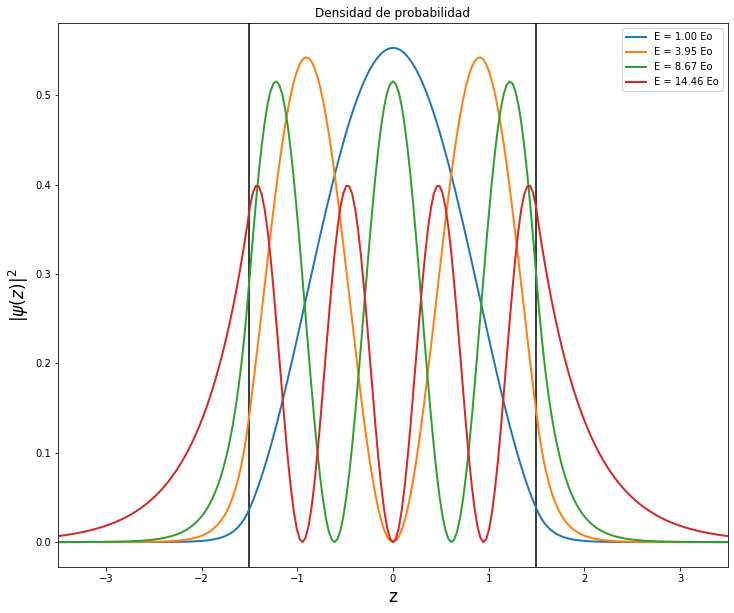
\includegraphics[width=0.50\textwidth]{finiteWallDensity.png}
\caption{Primeras 4 densidades de probabilidad para el Pozo finito de potencial}
\label{fig:finiteWelldensity}
\end {center}
\end{figure}

\begin{figure}
\begin {center}
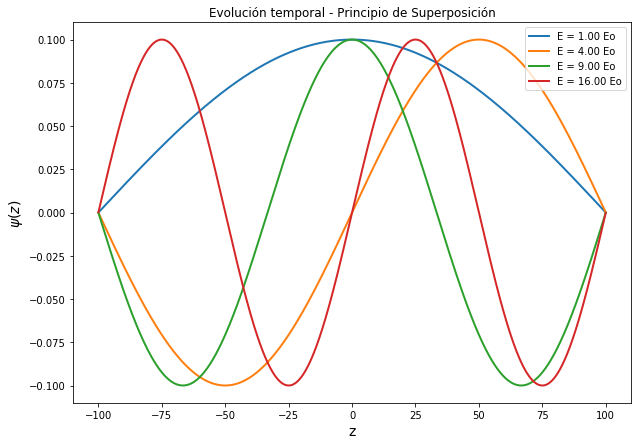
\includegraphics[width=0.50\textwidth]{infiniteWallPsi.png}
\caption{Primeras 4 densidades de probabilidad para el Pozo infinito de potencial}
\label{fig:infiniteWelldensity}
\end {center}
\end{figure}

\begin{figure}
\begin {center}
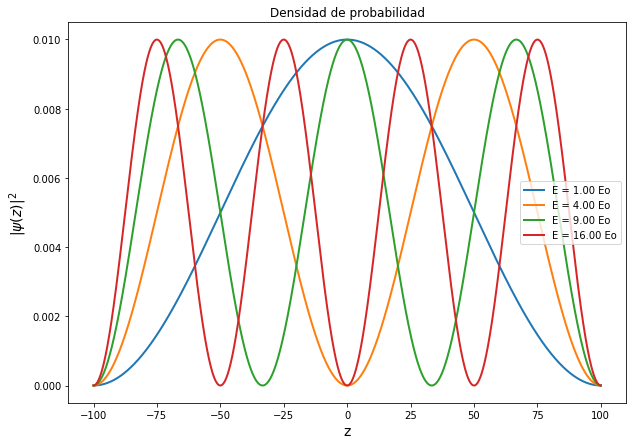
\includegraphics[width=0.50\textwidth]{InfiniteWallDensity.png}
\caption{Primeras 4 densidades de probabilidad para el Pozo infinito de potencial}
\label{fig:infiniteWelldensity}
\end {center}
\end{figure}

Al utilizar el principio de superposición, se ve que la densidad de probabilidad cambia con el tiempo, es decir, hay una evolución del sistema. El resultado es similar en el caso del pozo finito e infinito de potencial.

\begin{figure}
\begin {center}
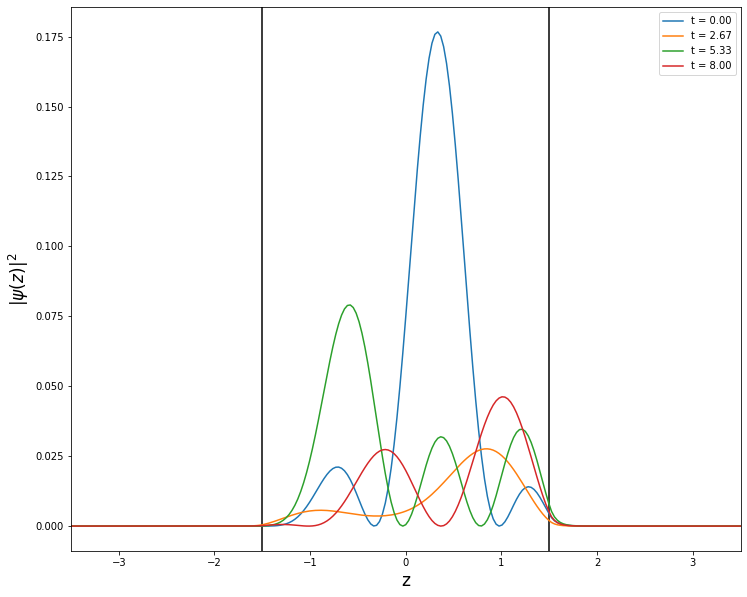
\includegraphics[width=0.50\textwidth]{finiteTemp.png}
\caption{Densidad de probabilidad del pozo finito de potencial para diferentes
tiempos.}
\label{fig:finiteTemp}
\end {center}
\end{figure}

\begin{figure}
\begin {center}
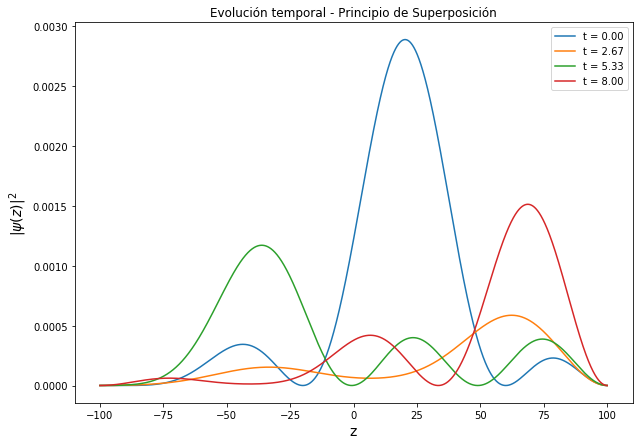
\includegraphics[width=0.50\textwidth]{InfiniteTemp.png}
\caption{Densidad de probabilidad del pozo infinito de potencial para diferentes
tiempos.}
\label{fig:InfiniteTemp}
\end {center}
\end{figure}

\end{document}